\documentclass[12pt]{article}
\usepackage[english]{babel}
\usepackage{natbib}
\usepackage{url}
\usepackage[utf8x]{inputenc}
\usepackage{amsmath}
\usepackage{graphicx}
\usepackage{subfig}
\graphicspath{{images/}}
\usepackage{parskip}
\usepackage{fancyhdr}
\usepackage{vmargin}
\setmarginsrb{2 cm}{1.5 cm}{2 cm}{1.5 cm}{1 cm}{1.5 cm}{1 cm}{1.5 cm}

\title{Pollination Contribution to Nutrition}								
\author{PolyScientists}
\date{\today}											

\makeatletter
\let\thetitle\@title
\let\theauthor\@author
\let\thedate\@date
\makeatother

\pagestyle{fancy}
\fancyhf{}
\rhead{\theauthor}
\lhead{\thetitle}
\cfoot{\thepage}

\begin{document}

%%%%%%%%%%%%%%%%%%%%%%%%%%%%%%%%%%%%%%%%%%%%%%%%%%%%%%%%%%%%%%%%%%%%%%%%%%%%%%%%%%%%%%%%%

\begin{titlepage}
	\centering
    \vspace*{0.5 cm}
    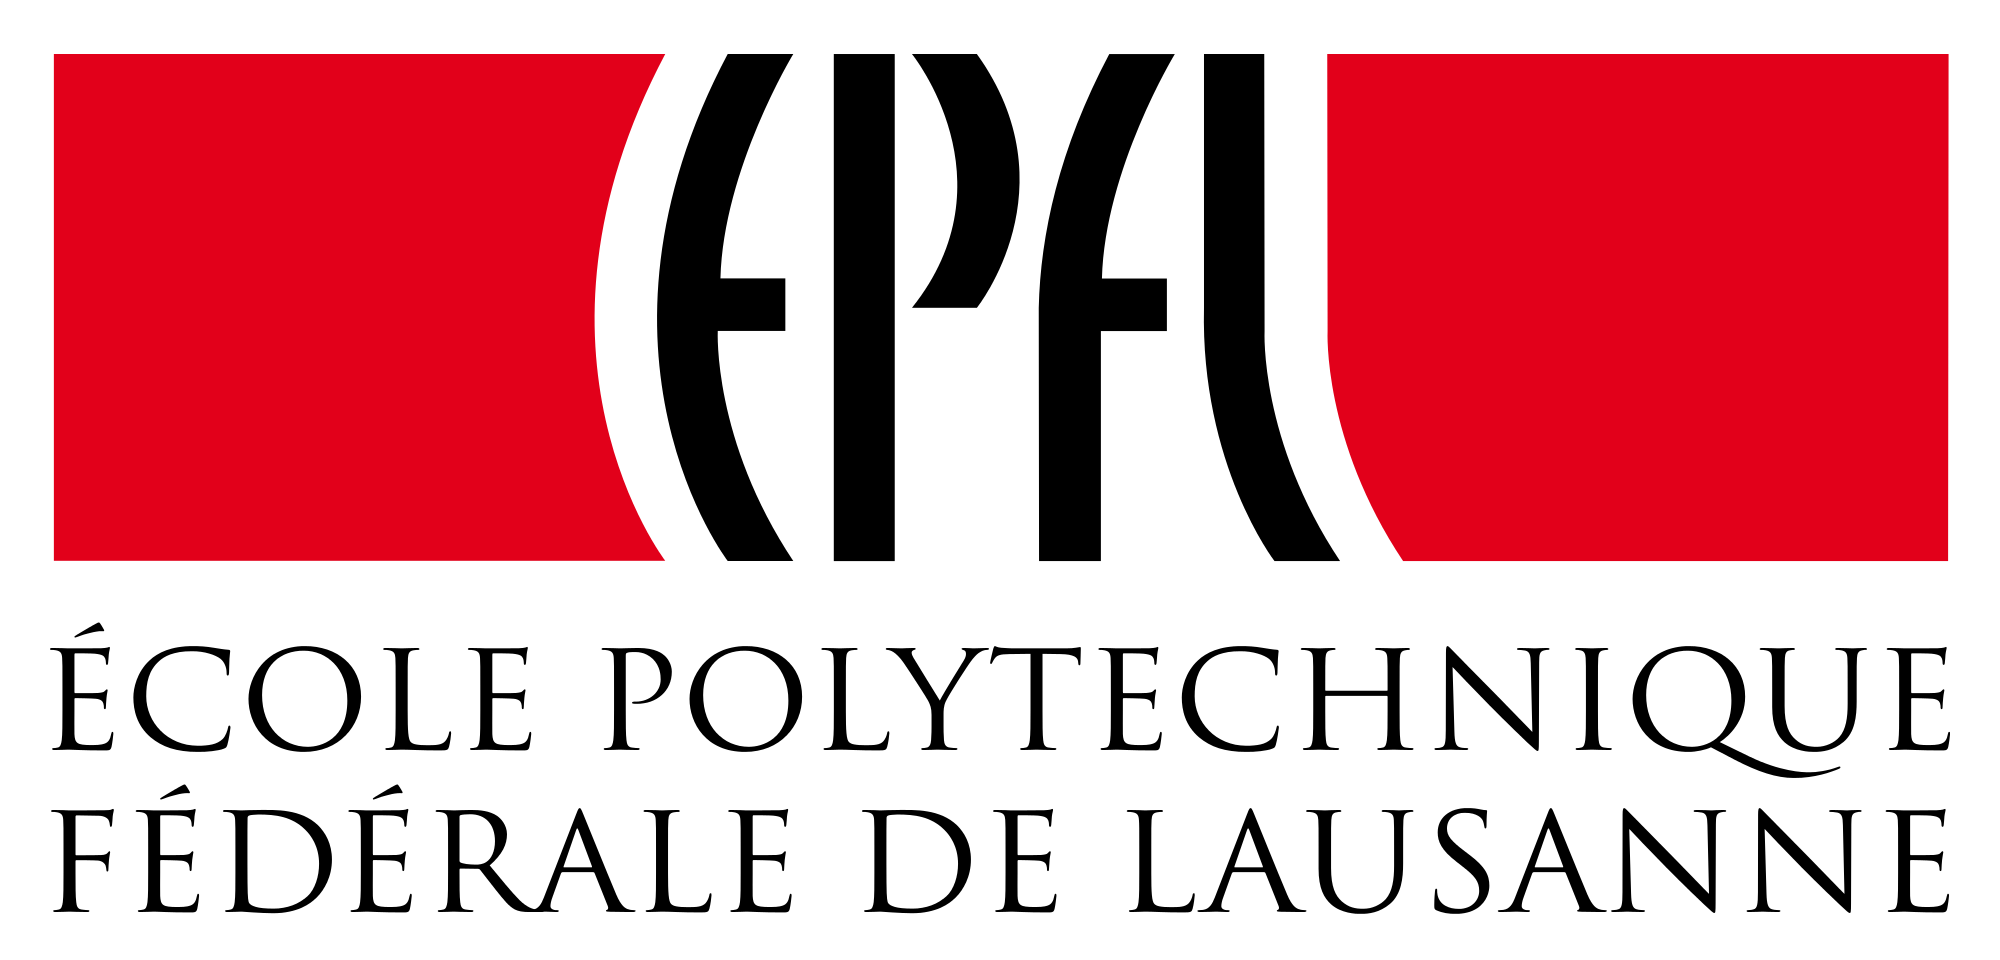
\includegraphics[scale = 0.11]{epfl_logo.png}\\[0.1 cm]	% University Logo
    \vspace*{0.8 cm}
	\textsc{\Large Data Visualization}\\[0.5 cm]				% Course Code
	\textsc{\large Process Book}\\[0.5 cm]				% Course Name
	\rule{\linewidth}{0.2 mm} \\[0.4 cm]
	{ \huge \bfseries \thetitle}\\
	\rule{\linewidth}{0.2 mm} \\[1.5 cm]
	
	\begin{minipage}{0.4\textwidth}
		\begin{flushleft} \large
			\emph{Authors:}\\
			Ahmed Ahres\\
			Sami Ben Hassen\\
			Harshdeep Singh\\
			\end{flushleft}
			\end{minipage}~
			\begin{minipage}{0.4\textwidth}
			\begin{flushright} \large
			\emph{Student Number:} \\
		    257294\\
		    237898\\
		    297332\\
		\end{flushright}
	\end{minipage}\\[2 cm]
	
	{\large \thedate}\\[2 cm]
 
	\vfill
	
\end{titlepage}

%%%%%%%%%%%%%%%%%%%%%%%%%%%%%%%%%%%%%%%%%%%%%%%%%%%%%%%%%%%%%%%%%%%%%%%%%%%%%%%%%%%%%%%%%

\tableofcontents
\pagebreak

%%%%%%%%%%%%%%%%%%%%%%%%%%%%%%%%%%%%%%%%%%%%%%%%%%%%%%%%%%%%%%%%%%%%%%%%%%%%%%%%%%%%%%%%%
\begin{abstract}
    The aim of this document is to showcase to the reader the process, design and implementation of the visualization focused on pollination contribution to nutrition. This project is the result of 7 weeks of intensive work and part of Stanford University's Natural Capital Project. The result is a visualization based on both a 3D globe and 2D map that showcases how pollination contribution is decreasing due to the decrease of wild pollinators, and how millions of people will be impacted in the future. 
\end{abstract}
\section{Introduction}
The goal of this process book is to detail the thought process behind the design and implementation of the visualization. This project is part of the Data Visualization course (COM-480) at EPFL. \newline
In this document, we present the concept of pollination, the data provided to us and the journey towards designing and creating a visualization centered around the pollination contribution to nutrition worldwide and how it will be affected in the future. Furthermore, we detail some of the implementation details and provide insights on what we have learned.
\subsection{Definition}
Pollination is defined as the transfer of pollen from the male part of the flower, the \textbf{stamen}, to the female part of the flower, the \textbf{pistil}. It is one of the most important processes when it comes to plant reproduction and is a crucial part of the eco-system. \newline
This transfer of pollen can be done by the wind, birds, mammals as well as insects; one of the most important insects are the honey bees that pollinate on a huge commercial scale. All sorts of fruit and vegetables are pollinated by honey bees, such as broccoli and squash, apples and almonds.
\subsection{Motivation}
It is estimated that 1/3 of the food is pollination-dependent, giving a large contribution of the pollinators towards our nutrition as human beings. However, one of the biggest obstacles that pollinators are facing today is the use (and misuse) of certain pesticides. Even though pesticides are not novel, new kinds of pesticides, called neonicotinoids, are harmful for pollinators [1]. With the increase of neonicotinoids usage comes a decrease in healthy pollinators thus negatively impacting nutrition in the world. Furthermore, the absence of an appropriate habitat for bees could lead to a continuous decline in pollination. Mono-cropping and higher temperatures associated with climate change all pose problems for bee populations and, by extension, the quality of food we grow. 
\subsection{Target Audience}
This project is part of Stanford University's Natural Capital Project (NatCap), which is a worldwide partnership among 250 groups developing a systematic approach to weighing nature’s benefits. This visualization will be used by a team of this organization (Becky Chaplin-Kramer, Charlotte Weil, Richard Sharp \& al) in the objective of helping communicate to the broader analysts community this work and its complexity. We also target any external user interested in the topic of pollination.
\section{Concept}
In the previous section, we have discussed the importance of pollination in the planet and the target audience of this visualization. In this section, we will be describing in details our dataset and showcase the several designs we came up with in order to visualize this dataset. Furthermore, we will show how our visualization went from a simple 2D map to two-level visualizations involving several complex components.
\subsection{Data-set}
During the beginning of the project, we were specifically asked to "spend time understanding the data as it is extremely complex". In this section, we briefly describe the dataset to the reader to understand what data is processed for this project. Due to the complexity and size of the dataset, we will describe only the sets that were used in the scope of this project.
\subsubsection{Exploratory Data Analysis}

The provided dataset is a large dataset containing various information about the pollination contribution to nutrition . The data is focused on three food nutriments: folate, vitamin A and food energy. Within these food nutriments, two main components are available:
\begin{itemize}
    \item Nature's contribution to Pollination (NCP) representing the pollination contribution to each of the food nutriments.
    \item Unmet need (UN) representing the unrealized pollination-dependent production (where natural habitat is insufficient to meet pollination needs, a.k.a pollination-dependent production loss).
    \item Dietary requirements representing for each country/region the requirements of the local population in terns of folate, vitamin A and food energy.
\end{itemize}
For each of these components, we were provided data about several periods since 1850. Most importantly, we were provided three different historical scenarios according to the "Shared Socioeconomic Pathways" that represent predictions in the year 2050 and are vital to our analysis: 
\begin{itemize}
    \item SSP1: Sustainability – Taking the Green Road.
    \item SSP3: Regional Rivalry – A Rocky Road.
    \item SSP5: Fossil-fueled Development – Taking the Highway.
\end{itemize}

\subsubsection{Data Description}
The data was provided using "labels" that were created by the NatCap team. The following labels were used: 
\begin{itemize}
    \item X1: Unrealized pollination-dependent production
    \item X2: Realized pollination-dependent production
    \item Y: Pollination-independent production
    \item Z: Local nutritional requirements
\end{itemize}
Using these various labels, we were able to compute the necessary data for our analysis. A very helpful document was provided to us by the NatCap team to explain the data more: 
\begin{figure}[htbp]
\centering
\includegraphics[scale = 0.35]{data.png}
\caption{Explanation of the data provided by the NatCap team.}
\end{figure} \newline
We have mainly used these labels to compute the pollination contribution to nutrition (through X1 and X2). \newpage
\subsection{Visualization Journey}
This section details the design and implementation of the visualization from the very early stages.
\subsubsection{Brainstorming \& Initial Sketches}
Before diving into the actual creation of the visualization, it is meaningful to go through a brainstorming session in order to come up with ideas. Initially, our goal was to present a 2D map containing other interactions (such as slider) to visualize the data. The following figures represent the first sketches created by the team.
\begin{figure}[htbp]

\centering
\includegraphics[width=220pt]{storytelling_first.jpeg} \fill
\includegraphics[width=220pt]{sketch1.jpeg}

\caption{Left: The storytelling section which comes right before the visualization. Right: The visualization section.}

\end{figure}

\subsubsection{Towards the First 2D Map}
In order to follow up on our initial inspiration, we designed and implemented the first 2D map with a slider to visualize the pollination contribution to Folate in the world (See figure).
\begin{figure}[htbp]
\centering
\includegraphics[scale = 0.15]{2dmap.png}
\caption{2D Map - Initial Visualization}
\end{figure} \newline
This visualization allowed the user to see the data in all the countries at the same time, while being free to select the period. The data updated in real-time with the slider. \newline
However, the first feedback we received was that too much space is "wasted", and more space should be dedicated to story-telling next to the map. As a result, we have decided to change our visualization to a 3D globe instead of a 2D map. This would then allow to have some space for the story-telling section, thus giving more insights to the user and understand what he/she is visualizing.
\subsubsection{A Shift to 3D Projection}
The D3 library has the advantage of easily allowing the change of projection. 
\begin{figure}[h]
\centering
\includegraphics[scale = 0.30]{3d_globe.png}
\caption{The 3D projection from D3}
\end{figure} \newline
This helped us build more space for other parts of the visualization such as storytelling, legend, information bar etc. \par

Initially, we were using the \textit{d3-geomap} library for the 2D Projection, and aimed to continue using it for the 3D globe as well. \newline
However we quickly realized that the library did not provide a lot of flexibility, thus limiting our ability to create a rich visualization. For instance, designing and implementing the ability to rotate the globe did not exist. This meant that more features in the future will potentially be hard to design and implement. \par

In order to circumvent this problem, we used the core function of the D3 library and constructed the projection. More details about this implementation are discussed in Section 3. \newline
While interacting with the globe, we have realized that the continent of Antarctica takes up a lot of space in the projection, without giving value to the visualization as the data was missing anyway. Hence, we decided to delete the continent of Antarctica. \newpage

\begin{figure}[h]
\centering
\includegraphics[scale = 0.20]{no_gradient.png}
\caption{The 3D globe with a real-time changing slider}
\end{figure} 

To make the globe look more realistic, we put an overlay of a blue circle at the back of the map which resembles the ocean. Furthermore, one key feedback comment was that the colors were not properly chosen. NatCap provided us with a document shown in [2]. Section 2.2.4 of this document states that \textit{"Sequential color scheme ought to be chosen when the underlying data shows ranked differences"}. However, our globe was using a diverging color scheme, thus not responding to data visualization principles. This has resulted in the following globe:
\begin{figure}[h]
\centering
\includegraphics[scale = 0.20]{3d_globe_2.png}
\caption{The globe with the blue gradient and new color scheme}
\end{figure} \newpage

At this stage, an initial version of the visualization part was completed. The result was a rotatable 3D globe presenting the user data about the contribution of pollination to Folate only. On the other hand, it was difficult for the user to understand what is being shown. Moreover, there was no way for the user to select whether Folate, Vitamin or Food Energy should be visualized. As a result, we needed a "panel" containing this possibility, and most importantly a story telling section.  
\subsubsection{Building up the Storytelling}
\textit{"Numbers have an important story to tell. They rely on you to give them a clear and convincing voice."} Stephen Few \newline

One of the fundamental aspects to make our visualization richer is story telling. By looking at the globe, the user cannot get any meaningful conclusions from it. It is our responsibility to make sure that the user understands what is being shown and be able to interpret the result. 

At the start, the story telling section was designed to contain data such as which country is zoomed in, the population and production of Folate, Vitamin A \& Food Energy. The design was, and still is, based on \textbf{hierarchical visualization}. More specifically, if the user is zoomed out, he/she can see the data for the world as to if they are meeting the food production or not along with the world population. But if the user clicks on a certain country, then information about the selected country is displayed.  \newline
\begin{figure}[h]
\centering
\includegraphics[scale = 0.28]{storytelling_v1.png}
\caption{Example of }
\end{figure} \newline
However, the feedback was that this section is too textual and not visual enough. This amount of text was not pleasing to read. Such a story-telling should contain more visual aspect to it to provide better insights to the user. 
A new version has been designed and is shown below:
\begin{figure}[h]
\centering
\includegraphics[scale = 0.20]{design-story.png}
\caption{Design of a second version of the story-telling, involving more visual aspects}
\end{figure} \newline
This new design contained three key features: 
\begin{itemize}
    \item It contained more visual aspect, thus responding to the feedback.
    \item It allowed for space to switch between the data to visualized. On the right hand side, F, VA and Energy respectively stand for Folate, Vitamin A and Food Energy. 
    \item It showed the user more information than only the different productions. This design showed the user the population, production, the contribution (an exact value of what is being shown on the map) and the unmet need. The unmet need corresponds percentage of pollination-dependent production loss. More specifically, it is how much production that depends on pollination is not achieved due to the lack of pollinators (due to lack of habitat or use of pesticides among other reasons).
\end{itemize}

\begin{figure}[!ht]
\centering
\includegraphics[scale = 0.20]{story_telling_2.png}
\caption{Implementation of the second design of story-telling, focusing on visual aspects}
\end{figure} \newpage
In this design, the percentages, population and production represent the data that are modified depending on the value in slider (the selected year) as well which country is selected. At the world level, the percentages presented to the user are the average of all the countries. \newline
While this was an improvement from the older version, it did not allow the user to easily see how the contribution decreases over the years, which is what this visualization wants to show. At this stage, the user had to manually change the slider value back and forth to be able to see how contribution actually decreases and the unmet need increases. \newline
In order allow the user to visualize these visualization, we have added a graph which shows the change of these data from 1850 up to 2050, resulting in the following story telling:
\begin{figure}[!ht]
\centering
\includegraphics[scale = 0.20]{final_story_3d.png}
\caption{Story telling with a focus on comparing different periods}
\end{figure} \newline
The added graph changes for each country and for each visualized nutrition. The figure above clearly shows that the unmet need increased heavily since 1850 and the pollination contribution has decreased since. The user has now the possibility to see, for the world or a specific country, how both of these variables have changed since 1850. \newline

At this stage, we had designed and implemented a rotatable 3D globe with a visual story-telling. The user has the ability to select the production to be visualized, and the story-telling changed accordingly. The overall visualization is shown in the following figure:
\begin{figure}[h]
\centering
\includegraphics[scale = 0.15]{3d_part.png}
\caption{Result for the 3D globe along with its story telling}
\end{figure} 
The feedback received from the NatCap team was that this visualization was "beautiful" but does not "show what we need". This has a resulted in a small shift of our perspective as a team, since the visualization did not allow for any analysis. This version was informative for a user to see how his country or any selected country he/she is interested in has changed since 1850. It was showing the user how pollination contribution has decreased and the unmet need has increased overall. It was well-designed for these purposes which analysts already knew, but not for more. 
\subsubsection{Towards a Visualization for Analysts - Adding a 2D Change Map}
The 3D globe designed and implemented was not very interesting for analysis purposes. While the visualization is enough for an external user to see how pollination is affected in the world, the target audience was not convinced with how much the visualization goes in-depth. For instance, having the 3D globe did not allow to compare the entire map since the globe did not show all the countries in the world. Additionally, we were not able to (easily) see how future scenarios compare with the current situation. Furthermore, we were asked to dis-aggregate the countries and only focus on the regions. Clearly, we needed to design a certain way to add more depth to the visualization. \newline
As a result, we decided to add a second part to the visualization centered around the 2D map, with the purpose of giving insights on 2 main points: \newline
\begin{itemize}
    \item Allow the analysts to compare the pollination contribution to nutrition in the entire world (i.e. be able to visualize all countries at once)
    \item Allow the analysts to see how future scenarios compare with the current situation
\end{itemize}
On top of the 2D maps, the story-telling needed to be updated. The story-telling section in the 3D section was designed for separate countries and show the difference since 1850 using historical data. However, this did not apply anymore. We needed a certain way of showing was is happening in the future. One of the suggestions received by the NatCap team is to visualize the number of people impacted per continents (or regions) in each of the scenarios. Following this suggestion and our creativity, this figure shows the design of the story-telling created by the team for the new visualization intended for analysts: 
\begin{figure}[h]
\centering
\includegraphics[scale = 0.20]{design-story-2d.png}
\caption{Design of the story-telling in the visualization intended for analysts}
\end{figure} 
Furthermore, since we will be using a change map, an important feature is to match the color scale used for the change to a \textbf{diverging} color scheme (as learned in [2]). Following this data visualization "rule", we have implemented the following 2D visualization. 
\begin{figure}[!ht]
\centering
\includegraphics[scale = 0.20]{2dview.png}
\caption{The 2D visualization}
\end{figure} 
This result contains an interactive bar graph to compare the number of people impacted by the selected period (SSP1, SSP3 or SSP5) in the different regions when hovering over one of the rectangles. We made this design decision since this allows an easier analysis between the different regions. Keeping in mind that this visualization is really designed for analysis purposes, this design decision made sense. \newline

Of course, this map would not make too much sense if there was no possibility to zoom and see certain parts of the map. Our goal is to really allow analysts to be able to see how contribution will change in the future. In this sense, we have added a possibility to zoom and travel through the map: 
\begin{figure}[!ht]
\centering
\includegraphics[scale = 0.20]{2dtranslate.png}
\caption{The ability to zoom and travel in the 2D maps to analyze how contribution will change in different regions.}
\end{figure} \newline
\subsection{Differences from the initial proposal}
The initial proposal was a very \textbf{minimalistic} version of what has been accomplished. At first, we aimed for a simple 2D map containing the pollination contribution data, with a somewhat visual story-telling. However, as explained in the previous section, several series of feedback have resulted in the design of a 3D globe for a better use of space, very visual story-telling for a rich visualization and not one but two 2D maps for comparison purposes.=

\section{Implementation}
In this section, we describe the technical details and challenges faced regarding the implementation of the visualization. We also describe the interaction that the user can perform with it.
\subsection{Technical Details \& Challenges}
Several libraries and frameworks have been used for this project:
\begin{itemize}
    \item The data processing was done using Python on a Jupyter notebook. Since the data was first provided to us a GeoPackage file, we used Fiona to copy vector data from the data source to Python objects as layers then used GeoPandas to create CSV files for the visualization.
    \item The visualization itself uses Javascript, D3, HTML and CSS.
    \item The link between Javascript and HMTL is achieved using jQuery.
    \item Various D3 libraries were used for small implementations. Examples are \textit{d3-simple-slider} for the sliders and \textit{d3-legend} for the several legends of the maps. 
\end{itemize}
During the development phase, four aspects have been particularly challenging, especially given the fact that the whole team are new to web development and Javascript: 
\begin{itemize}
    \item \textbf{Synchronizing the data:} One of the key components of this visualization is the change of data between periods using the slider, clicking on a particular country, selecting the data to be visualized (Energy, Folate or Vitamin) and the visualization selected by the user (2D or 3D). A high number of factors thus need to be taken into account each time. Some of the questions that arise when tackling this problem are: What is the user currently seeing? Is he zoomed in? How do we maintain the current data being visualized when he switches visualization? Which period is he in? \newline
    The data is continuously changing as the user interacts: the line graph in the 3D visualization changes with the country, the bar graph in 2D changes with the slider, the percentages displayed in the 3D version also change with the slider. \newline
    As a result, a lot of effort has been put in making sure that the data being shown is always the correct and expected one.
    \item \textbf{Creating the 3D globe:} As explained earlier, the switch from the 2D version to the 3D version at the beginning of the project was not as smooth as expected. We first started by looking at the "easy way": finding a library that does it for us. This was indeed successful at the beginning with the \textit{d3-geomap} library. However, we quickly realized that we were very limited with this library and the "easy way" will actually make the development harder at future stages. For example, the library allowed an easy change of projection, but made it complicated to have a smooth and realistic rotation. As a result, with the use of the \textit{inertia} library, we implemented the globe rotation by our own.
    \item \textbf{Smooth switch between visualizations:} The switch between the two visualizations has resulted in several bugs that needed quite some effort to fix. The simple switch using buttons was quite straightforward, however zooming in the 2D level then coming back to 3D for instance has created several bugs since a smooth zoom itself is not an easy task.
    \item \textbf{Responsiveness:} Another key aspect of our visualization (and of any visualization) is responsiveness. With the use of several flex-boxes, buttons and text to design the story-telling as well as the visualization itself, it became hard at the end to make sure everything is responsive and designed as it should be. As a result, a lot of effort and testing with several computers was done to ensure responsiveness. An example of non-responsiveness is shown in the following figure: 
    \begin{figure}[!ht]
\centering
\includegraphics[scale = 0.20]{bug.png}
\caption{The result of non-responsiveness}
\end{figure} \newline
    
\end{itemize}
\subsection{Interactions}
In this section, we provide the reader information about how to interact with our visualization using screen shots. \newline

\textbf{1.} At first, the user will be shown a pop-up window the explain the visualization.
\begin{figure}[h]
\centering
\includegraphics[scale = 0.15]{step0.png}
\caption{First interaction}
\end{figure}

\textbf{2.} After clicking on the \textit{Got it!} button, the user will be able to see the 3D visualization as a whole. The user can click on the globe and rotate it using the mouse.
\begin{figure}[h]
\centering
\includegraphics[scale = 0.15]{step1.png}
\caption{Rotation}
\end{figure} \newpage

\textbf{3.} When clicking on a particular country, the user can see more detailed data in the regions of the selected country. The story-telling will also update to represent the data about that particular country. By hovering over one region with the mouse, the user can see the data about that particular region.
\begin{figure}[h]
\centering
\includegraphics[scale = 0.15]{step2.png}
\caption{Zooming on the United States}
\end{figure} 

\textbf{4.} The user can see the data not only about the food energy, but also about vitamin and folate. In order to do so, the user can click on the corresponding button in the right side of the screen. The color will also be updated according to the color represented by the data. With this, the user will not "forget" what he/she is visualizing.

\begin{figure}[h]
\centering
\includegraphics[scale = 0.15]{step4.png}
\caption{Clicking on the "Folate" button.}
\end{figure} \newpage

\textbf{5.} The user can select the period to be visualized by dragging the slider under the globe. This will update the percentages shown in the story telling according to the selected period. 
\begin{figure}[h]
\centering
\includegraphics[scale = 0.15]{step5.png}
\caption{Selecting the year 1850}
\end{figure} 

\textbf{6.} The user can switch the view to visualize the "analysts" section. By clicking on the button on the right displaying a "map", the user switches the view. %
\begin{figure}[h]
\centering
\includegraphics[scale = 0.13]{2dview.png}
\caption{Switching the view}
\end{figure} \newpage

\textbf{7.} The user can zoom in the 2D maps by using the scroll and setting the cursor in the part the user wishes to zoom in. The user can also drag the cursor to move in both 2D maps and be able to compare.
\begin{figure}[h]
\centering
\includegraphics[scale = 0.13]{2dzoom.png}
\caption{Zooming in the 2D part. Note that the zoom is applied to the two maps.}
\end{figure}

\textbf{8.} The same interactions (slider and buttons) apply in this view. On top of this, the user can interact with the graph displayed in the story-telling section by hovering over one of the bars. This would then show, for each other continent, the difference in people impacted with the current selected one. The graph was made in a log scale in order to have a readable, yet informative visualization.
\begin{figure}[h]
\centering
\includegraphics[scale = 0.30]{graph.png}
\caption{Interacting with the bar graph. By hovering, we can compare the numbers in other regions. The numbers that are appear represent the difference between the currently selected region and the others in terms of millions of people}
\end{figure} \newpage

\textbf{9.} The user can then switch back to 3D by clicking on the button in the right side displaying a globe. 
\section{Evaluation \& Insights}
This section details the research questions we have answered and what we learned throughout the project.
\subsection{Research Questions \& Answers}
There is no point of having a data visualization if it does not teach or inform the user about anything in particular. It is vital to target research questions that the visualization should answer. In our project, we have aimed to answer the following research questions:
\begin{itemize}
\item How has pollination contribution to nutrition evolved since 1850?
\item Which countries/regions are mostly impacted by the decrease of wild pollinators?
\item How does the future of pollination look like?
\item How many people will be impacted by this?
\end{itemize}
We have aimed to analyze these questions by providing the user two visualizations. The 3D globe is mainly intended to analyze the pollination contribution to various nutriments at the country level. By having a line graph in the story-telling, we were able to show the user for the selected country or world how pollination contribution has changed since 1850. 
Furthermore, by having the change map in the 2D sections, we are able to easily analyze how future scenarios compare to the current scenario. \newline
Last but not least, the interactive bar graph allows an analysis of the number of people (in millions) that will be impacted in the future.

\subsection{What We Learned}
By completing this project, we have learned not only about the importance pollination but especially how the future unfortunately does not look bright for it. When starting this project, we only knew very few about pollination. As a team, we were only aware about what it is conceptually and the fact that it does contribute to food. \newline
However, we have learned a lot by visualizing this dataset:
\begin{itemize}
    \item The pollination contribution to nutrition has severely decreased since 1850 in most of the countries. This is due to only the increase use of pesticides, but also higher temperatures which leads to the loss of the pollinator's natural habitat
    \item The percentage of people impacted by this has heavily increased
    \item Analysts have already tried to predict the year 2050 in this context through the "Shared Socioeconomic Pathways" (SSP), which 3 scenarios exist: SSP1 for Sustainability, SSP3 for Regional Rivalry and SSP5 for Fossil-fueled Development
    \item Millions of people will be impacted in the future no matter the scenario, however SSP1 minimizes the damage
\end{itemize}
Furthermore, we believe that one of the key components that helped this project is \textbf{continuous feedback}. During the entire process, we have tried to receive as much feedback as possible by asking the NatCap team and staff members that take care of this course. Thanks to their feedback, we have been able to create a full data visualization that can not only inform the external user about the pollination contribution to nutrition but also help analysts in their work.
\section{Future Work}
Several improvements can be made to this visualization. First of all, the regions shown when we click on a country in the 3D globe do not have an exact position. Borders at the region especially seem to sometimes appear in the neighboring countries. Unfortunately, this was the result of the dataset provided to us. While those points were very accurate in the 2D version, they were not exact latitude and longitude positions (only 2 decimals) therefore causing inaccuracies. \newline

Furthermore, more improvements could be made at the story-telling level. For example, when viewing the 2D maps, it would have been helpful to visualize more graphs/plots to see what is the difference between future scenarios. At the moment, there is only an interactive bar chart showing the number of people impacted. \newline

With more expertise and time, this visualization can be improved and become a very helpful tool to analyze how pollination will be impacted in the future. \newline
In an honest and final note, we still have a lot of ideas to improve this project. Unfortunately, the limited time did not allow us to implement all ideas and we hope to have the ability to keep working on it. We feel that this project taught us a lot about the importance of pollination, how to design for analysis purposes, how to create a data visualization and especially how to think from the end-user perspective. 
\section{Peer Assessment}
\subsection{Ahmed Ahres}
"Both of my team members have done outstanding work and been extremely passionate about this project. I have never been in a group that is willing to spend so much hours and being this committed. When we started data visualization, we had no idea that this project was gonna be this complex yet fruitful to our learning. Both Harshdeep and Sami were very prepared for team meetings (sometimes doing more work than I even expected). I have come to realize this when Harshdeep finished implementing the 3D globe at 3am! They both contributed equally to this project and are extremely flexible. Honestly, it is one of the best groups I ever had the chance to work with."
\subsection{Harshdeep Singh}
"I am really lucky to have team members which were organized and cared about this project. The data and the task at hand were challenging but everyone continuously motivated each other to work hard; which I really liked and we definitely learned a lot not only technologically vise but also working more coherently in a team. Sami with his debugging skills and Ahmed with 'always wanting to work hard' approach definitely helped us do better as a group. They both contributed equally and communicated regularly to arrange meetings and discuss about the visualization as to how to proceed iteratively. By far one the best groups I have worked with this semester."
\subsection{Sami Ben Hassen}
"I had a blast working with this group this semester, I have never had the chance to work within a team that was this motivated about a project (maybe it is because of the Stanford prize). Ahmed and Harshdeep have done amazing work in order to make the best possible visualization in the short time period we had. Everyone was very well prepared for the meetings. The one thing I will never forget is the 'hackathon' session we did in the last two weeks before the deadline when we did a lot of peer programming. During this period, I have come to realize the importance of this software engineering concept since it has helped us progress in our debugging of the code a lot faster. This team is so good that we are planning to reunite next semester for other classes’ projects."
\section*{References}
[1] \textit{The Xerces Society for Invertebrate Conservation}, \newline \url{http://xerces.org/neonicotinoids-and-bees/} \newline 

[2] \textit{Natural Capital Data Visualization}, \newline \url{http://viz.naturalcapitalproject.org}
\end{document}